\chapter{\signpost: Internet-scale secure and scalable connectivity}
\label{sec:signpost}
\ifpdf
    \graphicspath{{Chapter3/Chapter3Figs/PNG/}{Chapter3/Chapter3Figs/PDF/}{Chapter3/Chapter3Figs/}}
\else
    \graphicspath{{Chapter3/Chapter3Figs/EPS/}{Chapter3/Chapter3Figs/}}
\fi

% In this chapter we explore application of the SDN technology in Cloud Computing.
% The availability of cheap cloud computing resources, boosted the development of
% a wide ecosystem of applications that aim to fulfil the needs of users to handle
% efficiently and ubiquitly personal information.  We term this use case of cloud
% computing as Personal Cloud. Applications like facebook,
% dropbox, google services~et.al.  abstract online user identity among devices,
% associate it with information, which is disseminated based on the user policy.
% Such services manage to simplify the way we use computers, but most of the times
% they employ mechanisms that undermine the security and privacy of users, while
% use network resources inefficiently. 

In this chapter we explore applications of SDN in Internet-wide inter-device
connectivity.  The work focuses on the problem of information control and
distribution between the devices of a user across the Internet; a mechanism we
term a Personal Cloud.  Currently Personal Clouds rely on centralised cloud
providers to establish Internet-wide connectivity due to limitations in
bidirectional connectivity, discussed in Section~\ref{sec:intro:motivations}. As
a result, users are subject to privacy threats and performance limitations. We
argue that users require a distributed, scalable and user-friendly naming
mechanism to enable Internet-scale user-managed Personal Clouds.  We propose
\signpost, an Internet-wide overlay network architecture that establishes
Personal Cloud functionality and provides continuous connectivity and controlled
security. The architecture consists of daemons running on end-user devices, that
can configure and run several off-the-self connection-establishing software
packages.  The proposed architecture employs a distributed negotiation protocol
between end-hosts, which scales the control complexity through control
distribution.

% The architecture provides two points of integration with legacy applications. 
% From the user perspective, the system integrates functionality on the
% network layer of the OS, thus providing backward compatibility with existing
% applications on the forwarding path. Additionally, the design provides a 
% user-friendly naming abstraction to devices, over the DNS protocol. DNS
% lookups for device names establish an API for applications to request from 
% the system the establishment of a path between 2 devices; a mechanism which we
% call {\it ``Effectful Naming''}.

% The propose architecture utilizes \of-enabled bridge and a
% local controller on each device. Each controller by default forwards packets as
% normal on the local network. The forwarding logic, though,  is augmenting
% through a distributed coordination protocol which permits nodes to negotiate
% possible connection opportunities and establish ad-hoc tunnels, enabling as a
% result an Internet-wide distributed control mechanism. 
% At the core of
% our design, we  the naming service host abstraction. Each device
% acquires a global domain name, while each name resolution triggers a connection
% engine, that tries to find the best possible bidirectional channel between the
% two nodes. The naming service uses the established
% DNSSEC extension, providing a fully authenticated and secure control
% mechanism among \signpost and applications. Further, the distributed nature
% of the naming hierarchy in the Internet permits seamless control distribution.

In order to understand the feasibility and performance of the proposed
architecture we develop a strawman implementation, that implements the core
control logic of the proposed architecture.  Additionally, it integrates support
for a number of network connection and notification services.  Currently,
\signpost supports SSH, OpenVPN, TOR, NAT-punch and Privoxy connection
mechanisms, while it can also propagate Multicast-DNS notifications across devices.

In this chapter, we present in Section~\ref{sec:signpost-introduction} the
motivation for this work, followed then by the key observations for our design
in Section~\ref{sec:sp-signpost}. In
Section~\ref{sec:signpost-architecture}, we present the architecture of our
strawman implementation and its integration with existing software. Finally, in
Section~\ref{sec:signpost-evaluation} we present a number of micro-benchmark
tests for our system and conclude in Section~\ref{sec:signpost-conclusion}.

\section{Personal Clouds}\label{sec:signpost-introduction}

% Numerous applications and protocols have been developed to fulfil Personal Cloud
% functionalities, such as remote desktop access, file sharing, remote login,
% remote printing etc.   Such applications extend the computer abstraction with
% mechanisms providing information and resource sharing between devices.  

In the recent years, the global increase in personal computer adoption has
transferred a large portion of our life in the digital domain. For example, a
portion of our labour is stored in digital format, like PDF and word processing
files, while a part of our social experiences maps to digital photo collections.
As a result, our physical presence has a growing digital counterpart. The main
user interaction medium with his digital presence is through his personal
computing devices. Nonetheless, the increase in the number of computing devices
per-user introduces new challenges in digital resource management.
Complimentary to their personal computer, users on average currently own and use
a tablet, a smartphone and a variable number of purpose-build computing units
for home entertainment and gaming.  Each user device often fulfils a specific
set of roles, thus requiring access only to a subset of the user digital
presence, but these roles are fluid and intercept.  For example, a smartphone is
primarily a communication device, but end-users may use it as a media player. In
the latter case, the smartphone and the home entertainment system provide
similar functionality to the user and require access to the same subset of his
digital presence. This transition from a single PC to multiple devices and the
concurrent digital footprint augmentation creates a user requirement for new
services providing global and homogeneous access and control of personal digital
information and resources. We call this abstraction the user \emph{Personal
  Cloud}. 

In the rest of this Section, we present existing approaches
providing Personal Cloud functionality~(Subsection~\ref{sec:sp-approaches}) and
discuss their functional limitations in order to define the design goals for our
\signpost system~(Subsection~\ref{sec:sp-challenges}). 
% and introduce readers to the
% \signpost framework~(Subsection~\ref{sec:sp-signpost}).

\subsection{Approaches} \label{sec:sp-approaches}

% Although reachability is reduced, Internet remains a highly performant and
% connected system; it interconnects billion of users and transports Terrabytes of
% information daily. This is achieved due to the predominant operational model of
% Internet services. Hosts in the common case connect to a small subset of the
% Internet space that provides access to popular information.  This model, which
% is called {\it Client-Server model}, is a natural result of the power-law
% chatacteristics of various social and engineering mechanisms. Internet network
% graph is a power law graph, due to its scalable hierarchical structure, while
% information popularity exhibits strong power law characteristics. 

Currently, partial Personal Cloud functionality is readily available in a number
of applications. Such applications provide a wide range of abstractions and each
has different network resource and connectivity requirements. We group these
approach in two distinct categories, based on the service architecure. 

\paragraph*{Decentralised Personal Cloud}

The requirement to share information and computing resources has been a core
application for computer networks since their conception. Currently the average
user has access to a large number of free software packages and protocols that
provide Personal Cloud functionalities, such as remote desktop access
(e.g.~Remote Frame Buffer protocol~\cite{RFC6143}), file sharing
(e.g.~NFS~\cite{RFC3530}, SAMBA file service~\cite{samba}), remote login
(e.g.~SSH~\cite{RFC4253}), remote printing (e.g.~IPP~\cite{RFC2911}) etc.
between devices. Such applications follow the client-server connection paradigm
and extend the computer abstraction to accommodate inter-device connectivity and
resource accessibility. A user can setup and manage the equivalent
services on his personal devices and enhance his user experience with Personal
Cloud functionality.  In addition, the network community has developed
mechanisms to ease the configuration of such services.  Multicast-DNS, UPnP and
ZeroConf protocols allow a user to seamlessly browse and access available
services upon connection to a network. 

Decentralised Personal Cloud applications enable users to fully control their
digital footprint in a privacy preserving manner. Data are stored on users
devices and the user has full control on the propagation of his information. 
Nonetheless, deploying such service in the Internet raises significant
scalability issues. We focus on three significant problems in Internet-scale
deployments. 
% : {\it
%  Connectivity}, {\it Authentication} \/and {\it Usability}. 

\begin{itemize}
  \item {\it Connectivity}\/: Current Internet architecture cannot accommodate
    globally accessible network services to all connected hosts, as we have
    discussed in Section~\ref{sec:intro:motivations}. As a result, the
    Client-server connection model of decentralised Personal Cloud applications
    cannot guarantee universal functionality.  End-users commonly connect to
    the Internet through edge networks optimised for outgoing connectivity,
    while ubiquitous middleboxes in the Internet may disrupt connectivity. For
    example, NATed networks, that scale connectivity on the edges of the
    network, limit incoming Internet connectivity for a significant number of
    devices and require manual configuration to expose services. In addition,
    mobile and enterprise networks employ firewalls to restrict publicly
    accessible services on connected hosts for security reasons.
  \item {\it Authentication}\/: Distributed Personal Cloud applications employ
    an inflexible authentication mechanism. Authentication is usually based
    on global or user-based pre-shared passwords and public keys. In order to
    grant access to a Personal Cloud service, the user must know a-priori
    the interest of another user to connect and enable access in
    the configuration of the service, while assuming available
    an out-bounds secure channel to negotiate access details. 
  \item {\it Usability}\/: Decentralised Personal Cloud applications introduce 
    configuration requirements which dim them inappropriate for inexperienced
    users. As we have already discussed in Section~\ref{s:home_social},
    the average end-user is highly unlike to engage in systematic
    service configuration, particularly if the configuration tasks are long and
    complex. Establishing connectivity through decentralised mechanisms is
    not straightforward. Functionality contains
    assumptions on the connectivity of the environment and users have to
    resolve to ``trial and error'' approaches to check which configuration
    can be effective in a specific environment. \\ 
    As an example, we describe the steps required to access files in a remote
    computer using the SSH service. Before the user is able to connect to a
    computer over SSH, he has to configure the service on his local machine, the
    security credentials on the server and firewall and NATbox deployed in the
    network. Additionally, if his public IP is expected to change over the
    course of a day, he needs to setup a mechanism to access the current IP
    configuration, like DynDNS~\footnote{\url{http://dyn.com/dns/}}\@.  This
    connectivity is subject to the ability of the user in the remote network to
    use the SSH protocol on the preconfigure port.  In case this is not
    possible, the user has to resolve to a different service.   
\end{itemize}

\paragraph*{Centralised Personal Cloud}

An alternative approach, which has been highly successful in the recent years,
uses third party cloud services to establish Personal Cloud functionality.  In
this group we consider applications like the Google service suite or Dropbox.
These applications provide a simple, intuitive and ubiquitous mechanism to
store and retrieve data in the cloud and define information sharing policies.
Centralised Personal Cloud applications have been highly successful as they
overcome the connectivity problems of the decentralised approaches, by using
cloud network and computational resources. In addition, their popularity is
further augmented by the social functionality, supported by some of these
applications. For example, Google Docs allow users to store online documents and
process them in parallel with a defined subset of their contact list.  Although
this approach can be characterised as successful in terms of functionality, some
of the properties are ambivalent and demotivate user engagement. 

\begin{itemize}
  \item{\it Identity}\/: Cloud applications provide an effective control
       framework to disseminate information between devices and users.  Users
       define access policies based on online identities and the service ensures
       secure information delivery.  User authentication mechanisms though
       introduce privacy concerns, since they can be used to identify and
       monitor users.  In~\cite{Krishnamurthy2009} the authors reports cases of
       personal information leakage to ad services from Online Social Networks,
       in order to detect and characterize individuals, and Facebook has openly
       verified the existence of such services~\cite{beacon-facebook}. 

\item {\it Performance}\/: The availability of large amount of computational
      resources in current cloud infrastructures provide user-acceptable
      performance, regardless the volume of processed data.  Although, this approach
      underutilizes the rich computational resources available in
      end-user devices on the edges of the Internet.  Two devices connected to
      the same subnet will experience bloated RTT values when they communicate
      through a cloud service, while public cloud storage cost and performance
      is orders of magnitude higher than the equivalent local network file services.
      In~\cite{Wittie2010}, authors report a significant impact on the 95th
      quantile network performance of cloud services, due to latency and packet
      losses incurred by the Internet.
      \todo{Add dropbox measurement study}\todo{tail at scale ref}

\item {\it cost}\/: Free cloud services, like iCloud and dropbox, 
  have an interesting economical model, which provides limited free service in
  order to augment user-base, accompanied by a weak SLA's.  If a part of the
  service is compromised and sensitive information is leaked, the service
  provider bears minimum obligation towards affected users~\cite{cnet-dropbox}.
  Such costs are not directly observed by the end-user, but they may impact
  significantly his social and work experience. 

\item {\it Availability}\/: Cloud services run on well connected infrastructures
      with a large number of network engineers ensuring security and
      performance. All devices can use such services over the Internet. However,
      the centralised architecture of such services introduce a single point of
      failure in inter-device communication. For example, two devices belonging
      to different users and connected to the same local network cannot exchange
      a file over Dropbox, if the firewall policy forbids connectivity with the
      Dropbox servers~\footnote{Dropbox provides local network synchronization
        functionality between devices, but the users must have enabled their
        sharing policy a-priori and through the online Dropbox service}. 

% \item {\emph Generality}\/: Cloud applications develop distributed services
%       optimized for specific functionality. Google Drive provides online
%       document storage, Youtube provides online video hosting and Facebook
%       provides Online Social Network Services. Users are limited on their ability
%       to share information or resources by the offered capabilities of the
%       service provider and there isn't a sole service provider that can
%       support functionality for the complete ensemble of Personal Cloud services. 
\end{itemize}

\subsection{Design Goals} \label{sec:sp-challenges}

% In our exploration in Personal Cloud frameworks, we categorized Personal Cloud
% applications in two broad groups, based on their network architecture, and
% discussed their capabilities and limitations. 
In the previous section we present the capabilities and limitations of existing
Personal Cloud applications. Decentralized Personal Cloud configuration is
complex for an average user, while the functionality depends on the network
environment properties. On the other hand, centralised Personal Cloud
applications provide better usability, but they incur privacy
vulnerabilities~\cite{facebook-nsa} and functionality bottleneck.  

We believe that an efficient and secure Personal Cloud framework, should rely on
a hybrid approach to scale the problems of connectivity, security and usability.
User information should be stored on end-devices, to ensure user privacy, and
existing decentralized applications can provide Personal Cloud functionality.
Scalable inter-device connectivity can achieved through an evolved network
control plane on the end-devices. In addition, the user must maintain a globally
accessible service in the cloud, which enabled an global control channel between
the devices of a user. The service is used to aid end-device to bypass network
restrictions, but the system can function, up to a point, without interaction
with the cloud service. We set the following high-level goals for our network
architecture:

\begin{itemize}
  \item {\it Connectivity}\/: The framework should establish a new
    control abstraction, focused on the inter-device communication
    requirements of the user. This abstraction decouples the data flow of
    the application from the network state, enabling the implementation to
    choose at run-time the most efficient network mechanism to establish
    a communication channel. Additionally, the implementation of the
    connection abstraction should be able to automatically “self-heal“ 
    during network disconnections.

  \item {\it Control}\/: Individuals should control access to their devices.
    Access policies should operate on the level of devices or users and rely on
    strong authentication and encryption mechanisms. Additionally, the
    control should be sufficiently dynamic to respond to environment 
    changes, e.g.~propagate trust revocation for a compromised device. In
    addition, the control abstraction should consider multiple 
    security aspects and allow the user to control the trade-off between
    performance and security.
   
  \item {\it Backward Compatibility}\/: The framework should provide support
    to existing decentralised applications without any modification
    of their functionality.

  \item {\it Usability}\/: The system should expose a simple control abstraction
    to end-users and encapsulate all low-level interactions. Ultimately, the
    abstraction of the system should be compatible the existing user experience
    of decentralised Personal Cloud. 
    
%    Individuals need to have a memorable way to refer to devices. 
%    The naming service should dynamically adjust to the state of devices, provide global
%    coverage, be scalable and provide some partial mechanisms to obfuscate users
%    connection interest toward other entities. Additionally, the naming service
%    should provide a mechanism to detect unauthorized users as well as protocol
%    modifications.

 \end{itemize}

% Personal cloud computing requirements currently experience a mismatch with the
% functional properties of the Internet.  Personal devices usually connect to
% networks optimised for outgoing connectivity and various components of the
% Internet are not designed to accommodate well-connected services for every host.
% NATed networks, that scale connectivity on the edges of the network, require
% manual configuration in order to host Internet-reachable services, while a
% number of edge networks, namely mobile and enterprise networks, restrict
% publicly accessible services on connected hosts for security reasons. In order
% to overcome these restrictions a number of approach has been proposed by the
% research community, as well as the industry.  We group these solutions in the
% following two categories:

% Internet is an excellent example of a dynamic system managing to address
% effectively evolution.  In the early days of the system, in
% order to extend user adoption, its  steering committee set simplicity and
% openness as two fundamental design goals. Due to these design choices, Internet
% protocols gained rapidly support by a wide range of OSes, while the set of
% connected entities augmented exponentially.  Nonetheless, during that period, the
% Internet remained a large wide area network, interconnecting research
% institutes, and the predominant applications provided constraint relaxed
% asynchronous communication. Through the years though, and as Internet users
% increased, new applications emerged and highlighted a number of
% security and performance limitation in the initial design of the system.
% 
% In order to address these limitations in a backward compatible manner, a number
% of network hacks were introduced in the Internet design. One of the most popular
% hack is the deployment of middleboxes~\cite{RFC3234}.  Middleboxes violate in a
% number of ways design principles of the Internet, in order to provide an
% effective framework to ``inject`` functionality that addresses design
% limitation. For example, \emph{NATboxes} handle the IPv4 address space shortage,
% \emph{WAN optimizers} improve utilization of under-provisioned links, while
% \emph{firewalls} secure critical networks.  Unfortunately, Middlebox deployment
% redefines to a great extend the Internet abstraction. A number of papers have
% described their impact: in~\cite{Honda:2011ci} authors pinpoint middlebox
% functionality as a core cause in the ossification of the transport layer, while
% in~\cite{Kreibich10} authors describe a wide range of protocol functionality
% that has become suppressed due to middlebox functionality. 
% % Mainly, due to middlebox functionality, the
% % initial design properties of the system in terms of simplicity and openness have
% % been lost for a large subset of the Internet.  
% 
% \todo{ describe some efforts to overcome middleboxes.}
% \todo{IPv6 can do some of that,but not everything }
% An important impact of middlebox deployment is the reduced connectivity
% introduced in the Internet. Home networks host a number of hidden devices which
% remain inaccessible from the Internet due to NATbox functionality, while strict
% firewall policies in enterprise networks reduce protocol functionality.
% Personal Cloud deployment across the Internet is increasingly restricted, as
% devices are not able to interconnect directly.


\section{Finding your way with \signpost}\label{sec:sp-signpost}

\signpost is a Personal Cloud-enabling framework with user controlled security.
The system establishes an Internet-wide overlay network between the devices of a
user. The abstraction relies on a cloud-based control channel established
between devices which can be used to negotiate and establish
end-to-end connections, using existing decentralized frameworks. In order to
ensure functionality under any circumstance, we integrate the control channel
with the DNS protocol, an existing high availability and resilient service. 

The system establishes a user friendly framework that automates end-to-end path
configuration between devices.  \signpost models existing connectivity
mechanisms and encodes their configuration and assumption testing in a generic
automation framework.  Additionally, the system provides seamless integration
with existing applications. \signpost network paths are exposed in the network
layer of the OS and  the control API for inter-device connection establishment
is integrated with the \textit{gethostbyname()} function.  Each device is
exposed to the users as a domain name and a name lookup for a device triggers
the connection establishment mechanism. Inter-device traffic, destined to the
DNS-provided IP, is routed through the established path.  Finally, the system
exposes a user-controlled security abstraction, which can provide different
security properties on connections between devices. As a result, the user is
able to fully control the dissemination of information between his devices,
while avoiding privacy-sensitive data offload to cloud services. 

\begin{figure}[ht]
  \begin{center}
	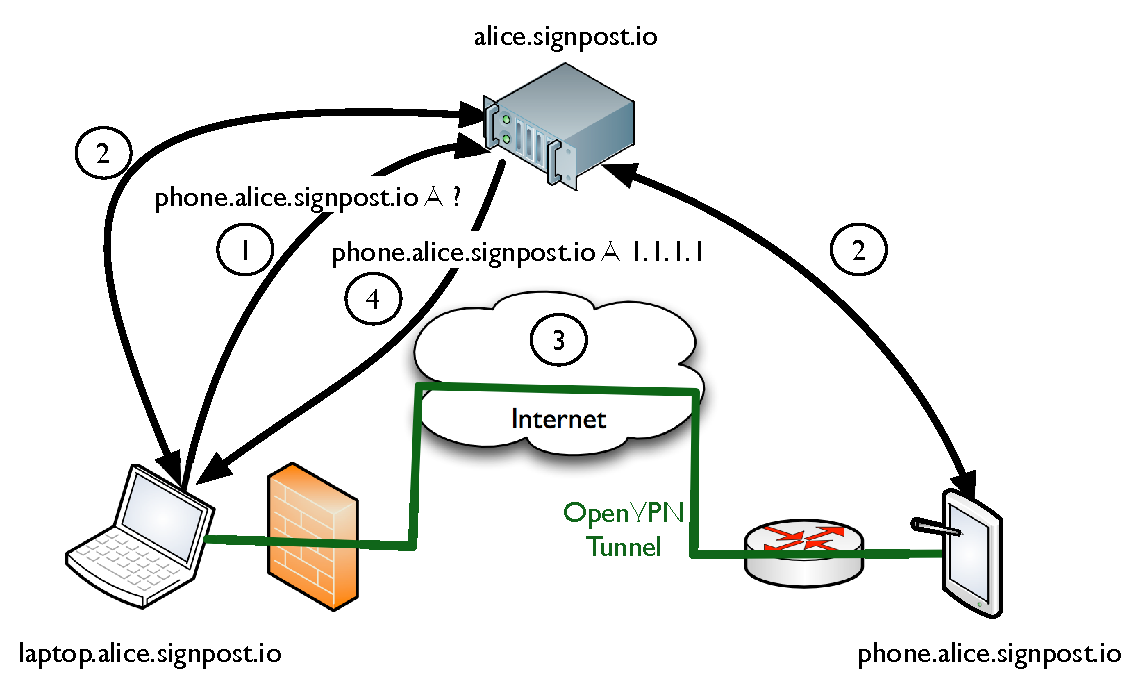
\includegraphics[width=0.6\textwidth]{Chapter3/Chapter3Figs/sp-illustration}
  \end{center}
  \caption{A simple example of the \signpost abstraction when the user Alice
    interconnects a smarthphone with the home computer over the Internet.}
  \label{fig:signpost-user-abstraction}
\end{figure}

\todo{Add some reference to cloud controller}
A schematic of the abstraction that our system provides to end-users is depicted
in Figure~\ref{fig:signpost-user-abstraction}. In this scenario user Bob, who is
at work and uses his smartphone, wishes to access some files on his laptop,
which is behind the NATed home router. In order to express his interest to
connect to his laptop, Bob must perform a name lookup for the domain name
\fqsn{laptop.bob} (step~\ding{192}). The name lookup will propagate through the public DNS service
to the cloud presence of her \signpost system, which we call the {\it \signpost
  controller}. The \signpost controll will trigger the two devices to try
multiple possible connection establishment mechanisms and setup an end-to-end
path between the two devices (step~\ding{193}). Once the server has ensured that a first path is
available (step~\ding{194}), it will reply to the initial DNS query with a local IP address which
will be routed by the local network stack to the tunnel between the two devices
(step~\ding{195}).
In parallel, the server will continue recursively to test different tactics, to
discover more efficient connection mechanisms. 

% Our work builds on the observations on the shortcoming of current approaches to
% interconnect devices, and tries to bridge the two domains, providing the
% appropriate control mechanisms to end-users. On one hand, we want to
% model a generic framework that will allow end-host to automatically test the
% network environment, discover the optimum mechanism to interconnect two
% devices and distributely negotiate the connection parameters with other devices,
% without any user interaction. On the other hand, we want to provide to the users
% a mechanism that will allow them to control to a great extend the security and
% privacy of their information. 

% §develop and deploy various protocol modifications that tried to bypass these
% design flaws.  Unfortunately, such systems tend to introduce stricter
% assumptions on how the network should function, and reduce to a great extend the
% openess of the Internet.There are primarily two major classes of engineering
% modifications that reduce network connectivity: performance enhancing
% middleboxes and edge-network security policy reinforcement.  
% Performance
% enhancing middleboxes are network forwarding devices, installed in the network,
% that aggregate information from multiple layers of the TCP/IP stack and modify
% packet content or forwarding logic. 
% This restriction in openess of some parts of
% the Internet is a vital reason for the inability of the network community to
% establish Private Clouds across the Internet.  


% \section{\signpost Design Goals} \label{sec:signpost-goals}

\section{\signpost Architecture}\label{sec:signpost-architecture}

\begin{figure}
  \begin{center}
	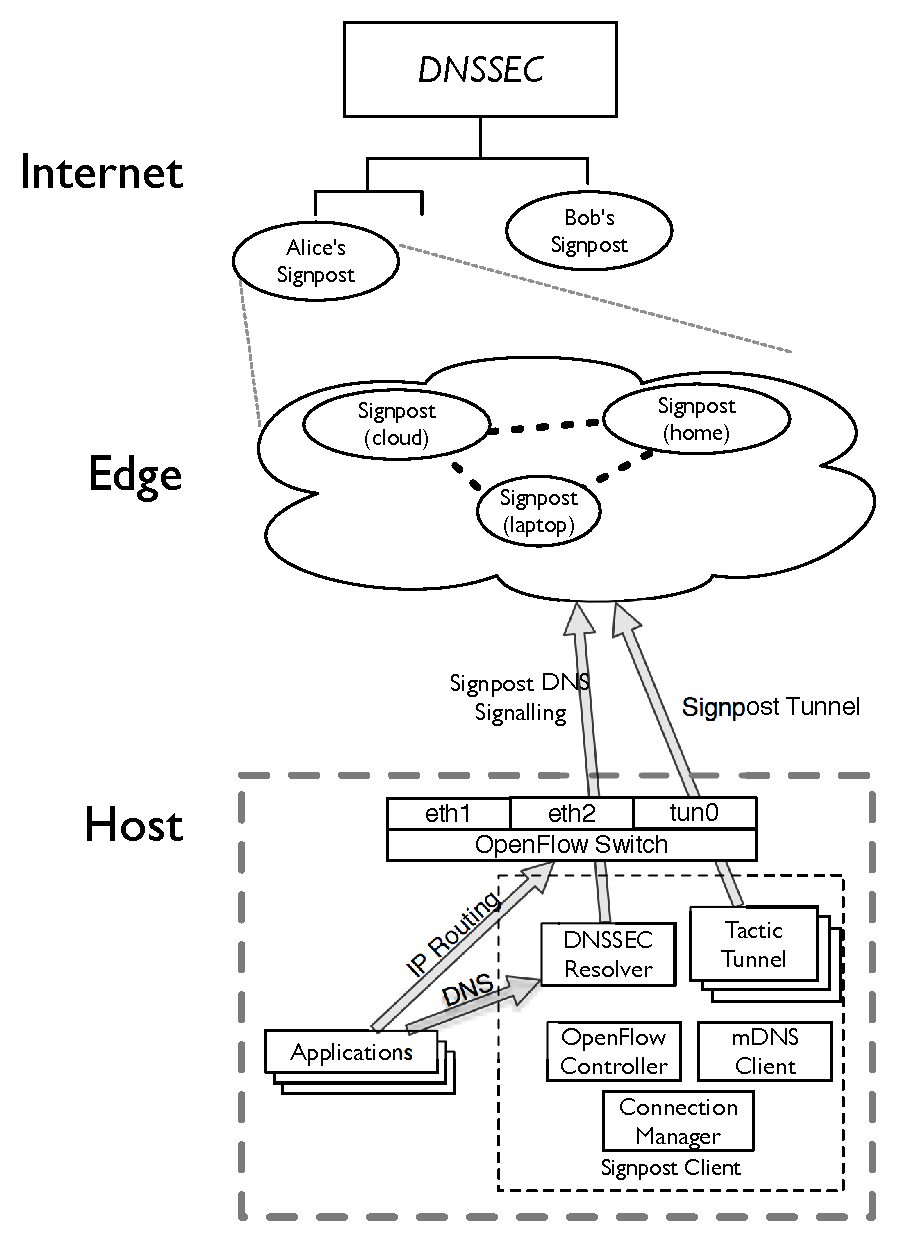
\includegraphics[width=0.9\textwidth]{signpost-arch}
  \end{center}
  \caption{\signpost architecture}
  \label{fig:signpost-arch}
\end{figure}

\signpost is an Internet-wide secure inter-device communication system. The
system reuses existing Internet protocols and connectivity mechanisms and
provides an overlay local network. In Figure~\ref{fig:signpost-arch} we present
a diagram of the \signpost architecture over different abstractions. 
%%
In the lower section of Figure~\ref{fig:signpost-arch}, we present the design of
the \signpost software and its integration with existing applications.
\signpost logic is contained in a single executable, and requires from the guest
OS to expose an OpenFlow switch interface and redirect DNS queries to the
embedded DNS resolver.  The software consists of three main subsystems: A
{\it Connection Engine}~(Subsection~\ref{signpost-engine}) that sets up and
manages {\it Network Tactics}~(Subsection~\ref{signpost-tactic} in order to establish
end-to-end paths, a local DNS resolver and an \of-based {\it \signpost
  router}~(Subsection~\ref{signpost-forwarding}) that enhances the normal OS
routing functionality with \signpost logic.  
%%
In the middle layer of Figure~\ref{fig:signpost-arch}, we present the control
plane interconnection of \signpost devices. The system relies on an
Internet-wide inter-device control channel, which enables capability and
parameter negotiation for end-to-end connectivity. The architecture considers a
\emph{Controller \signpost} instance running on a well connected host, which
bridges the device control channel across the Internet.  Further, the system can
establish connectivity between local devices without the mediation of the
\signpost Controller.  \signpost clients contain a Bonjour-based discovery
mechanism, through which devices can establish ad-hoc secure and authenticated
paths.
%%
In the upper layer of Figure~\ref{fig:signpost-arch}, we present the naming
organisation of the \signpost architecture. The system reuses the naming
abstraction of the DNS service. Each device has a global domain name, while the
domain hierarchy and name aliasing expresses the control relationship between
devices and users.  We extend the normal name resolution functionality of the
DNS protocol and introduce the  {\it Effectful name resolution} operation for
\signpost-enable domains; a name resolution expresses the interest of a user to
establish an end-to-end path~(Subsection~\ref{signpost-naming}). For the rest of
the section we present in depth the details of the \signpost system. 

\subsection{Network Tactic} \label{signpost-tactic}

\begin{table*}
\centering \footnotesize
\begin{tabular}{|l|c|c|c|c|c|c|p{1.5cm}| }
  \hline
  Tactic name & Purpose & Layer & Transport & Auth. & Encrypted & Anon. & \signpost
Support\\
 %% & Comment & Source \\
\hline
Avahi       & Discover         & 7      & UDP         & No     & No     & No & Yes\\
 %% & Linux-based, bonjour-compatible system for local network resource discovery
 %% & \url{avahi.org/} \\
Samba       & Discover         & 7      & UDP         & No     & No     & No & No \\
 %% & Windows local network resource discovery protocol, implemented in WINS & \\
Bonjour     & Discover         & 7      & UDP         & No     & No     & No & Yes\\
 %% & Used for local network resource discovery
 %% & \url{developer.apple.com/opensource/} \\
Universal PnP & Discover         & 7      & UDP         & No     & No     & No & Yes\\
dns2tcp     & Tunnel             & 7      & UDP         & No     & No     & No & No \\
 %% & IP over DNS & \url{www.hsc.fr/ressources/outils/dns2tcp/index.html.en} \\
DNScat      & Tunnel            & 7      & UDP         & Yes    & No     & No & No \\
 %% & VPN with PPP & \url{tadek.pietraszek.org/projects/DNScat/} \\
HTTP-Tunnel & Tunnel            & 7      & TCP         & No     & No     & No & No \\
 %% & uses HTTP & \url{www.nocrew.org/software/httptunnel.html} \\
iodine      & Tunnel            & 7      & UDP         & Yes    & No     & No & Yes\\
 %% & IP over DNS & \url{code.kryo.se/iodine/} \\
NSTX        & Tunnel            & 7      & UDP         & No?    & No     & No & No\\
 %% & IP over DNS. Deprecated. Recommends iodine 
 %% & \url{thomer.com/howtos/nstx.html} \\
% IMAP        & Data transfer     & 7      & TCP         & Can be & Can be & No \\
 %% & & \\
Proxytunnel & Tunnel            & 7      & TCP         & Can be & Can be & No & No\\
 %% & can use both HTTP and HTTPS & \url{proxytunnel.sourceforge.net/} \\
ptunnel     & Tunnel            & 4      & ICMP        & Yes    & No     & No & No\\
tuns        & Tunnel            & 7      & UDP         & &        No     & No & No\\
 %% & IP over DNS. Doesn't split IP packets, but sets size so small that OS does
 %%   fragmentation. Neat. Only uses CNAME for maximum compatibility with
 %%   infrastructure. Poor performance :( 
 %% & \url{www.loria.fr/~lnussbau/tuns.html} \\ 
SSH         & Tunnel/Encrypt & 7      & TCP         & Yes    & Yes    & No & Yes\\
IPSec       & Tunnel/Encrypt & 3 (4*) & IP          & Yes    & Yes    & No & No\\
 %% & In layer 4 when traversing NATS (over UDP or TCP) & \\
OpenVPN     & Tunnel/Encrypt & 7      & UDP/TCP     & Yes    & Yes    & No & Yes\\
 %% & & \url{openvpn.net/} \\
libjingle   & Nat punch         & 7      & UDP/TCP     & Yes    & ?      & No & No\\
 %% & For punching holes. Negotiation over XMPP
 %% & \url{code.google.com/apis/talk/libjingle/index.html} \\
privoxy     & Anonymize         & 7      & TCP         & ?      & ?      & Yes & Yes\\
tor         & Anonymize         & 7      & TCP         & No     & Yes    & Yes & Yes\\
 %% & & \url{www.privoxy.org} \\
% SMTP        & Data transfer     & 7      & TCP         & Can be & Can be & No \\
stunnel     & Encrypt        & 7      & TCP         & Yes    & Yes    & No & No\\
TCPCrypt    & Encrypt        & 4      & TCP         & No     & Yes    & No & No\\
\hline
\end{tabular}
\caption{\label{tbl:signpost-tunnels}Tactics table.}
\end{table*}

Currently the network community offers a wide selection of software to establish
connectivity between network devices. In Table~\ref{tbl:signpost-tunnels}, we
present a small survey of such mechanisms along with their network requirements
and security properties.  The table entries exemplify the high diversity among
the available connection mechanisms.  For example, a significant subset of the
mechanisms utilize application layer protocol functionality in order to establish
IP connectivity, thus allowing users to bypass strict network policies. An
equally significant subset of the mechanisms focus on encryption and privacy
enhancement of end-to-end Internet paths, while a third class of these
mechanisms enable connectivity through simple service advertisement. Further,
the mechanisms vary significantly on the employed network protocol and the 
connectivity they provide.  Tunnels provide connectivity on a specific port of
the transport layer, or introduce an overlay network on the network layer.  The
majority of the tunnelling mechanisms use UDP or TCP connectivity, while
there are protocols that function user other network protocols, like ICMP.
Finally, user authentication is variable.  Approaches vary from
user-based authentication using either passwords or certificates, to simple
Pre-shared passphrases, while a subset of the protocols luck authentication support. 

\begin{figure}
  \begin{center}
	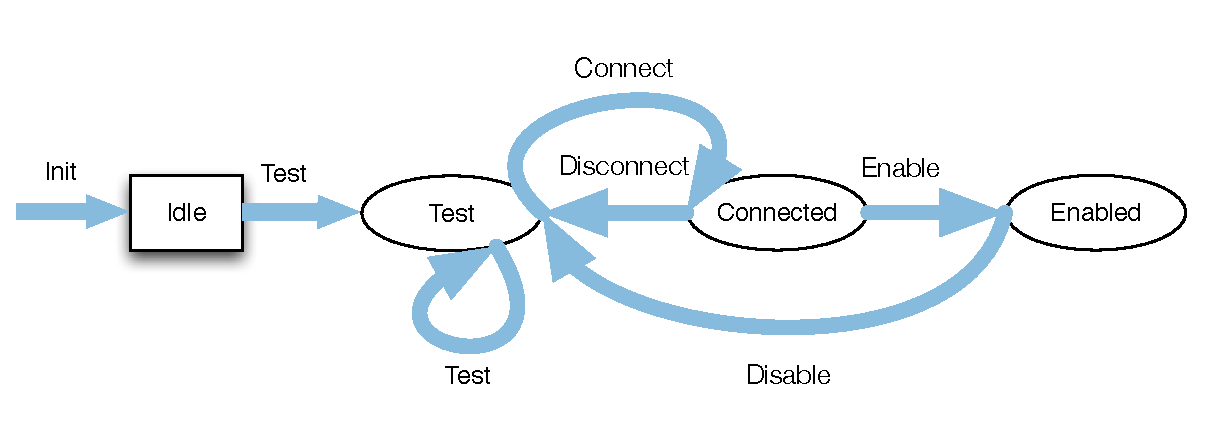
\includegraphics[width=0.6\textwidth]{signpost-tactic}
  \end{center}
  \caption{\signpost tactic lifecycle}
  \label{fig:signpost-tactic}
\end{figure}

In the \signpost architecture we model network mechanism 
functionality through a simple abstraction, which we term a
{\it Network Tactic}. A sufficiently generic specification of this abstraction
is core for the establishment of an automated connectivity platform.
% This abstraction enables modularization during the integration of new mechanism,
% while enabling the development of algorithms that optimize specific indexes on
% the exploration of the optimal combination of tactics to fulfil a user
% connection policy.
\signpost Network Tactics are modelled as a 4 state automaton.  The state space
diagram is presented in Figure~\ref{fig:signpost-tactic}. A Tactic initializes
in the Idle state. A test method invocation transfers the tactic to the testing
state, while executing the testing logic of the tactic. The test method performs
Tactic specific testing to detect network environment limitations and required
connectivity configuration.  If testing is successful, the Tactic can progress
to the connect state which will configure an end-to-end path. Once the
end-to-end path is established, the Tactic can progress to the enabled state and
forward packets over the path.  Finally, the Tactic automaton provides methods
to backtrack from each state and clear stored state. In order to avoid packet
reordering, \signpost permits the parallel existence of multiple connected
tactics for a set of devices, but a single tactic can be enabled at any point. 
\todo{rewrite last 2 sentences}

\signpost defines a generic model to split functionality between the \signpost
controller and client for a specific tactic in order to distribute control.  The
functionality of a \signpost tactic is split logically in two layers: the
Southbound layer, implementing low level tactic operations, and the Northbound
layer, translating the tactic abstraction into low level operations.  The
Northbound functionality runs on the \signpost controller, while the
Southmodule functionality runs on the \signpost clients. The two layers
of the tactic, communicate over the control channel using a tactic specific
protocol. 

As an example of this functionality split, we present the Test method of the
\openvpn tactic, an IP tunnelling system that uses certificate-based
authentication and functions over TCP or UDP\@. In the test section of the
Southbound layer, the tactic implements two methods: {\emph init} an \openvpn
server with default configuration and {\emph test} if an \openvpn server is
accessible on a given IP and port. The Northbound layer of the tactic expose a
single test method, which instructs participating devices to initiate an
\openvpn server and test client connectivity towards the other device. The first
client returning a successful test result becomes the client of the \openvpn
tunnel while, if the test times-out for both devices, then the controller
initialises an \openvpn server and instructs the devices to test \openvpn
connectivity to the controller.

% In the development of the 
% we also consider the way that the
% design can encapsulate the complexity to address the problem of increased
% heterogeneity of the level of connectivity that a Network Tactic provides, we
% include two equally important details in the abstraction. Firstly, each tactic
% can directly modify the forwarding table of the OpenFlow Switch and receive
% feedback from the forwarding plane. In this way we can incorporate in the
% architecture tactics that provide port-based connectivity, as well as network
% layer connectivity. Secondly, because we are interested to allow user
% flexibility on the properties Tactic synthesis in order to enable complex
% combinations of Tactic that can fulfil user policy, we introduce in the design a
% simple mechanism to express meta-data informations on the connection
% requirements of a 

\todo{Discuss weight of tactics}

\subsection{Forwarding} \label{signpost-forwarding}

\todo{talk in abstract ot explain specific}
We integrate \signpost functionality at the network layer of the host for strong
backward compatibility with existing decentralized applications. A \signpost
cloud is abstracted as a local subnet and persistent local IPs are allocated to
devices. In addition, \signpost clients must expose a flow forwarding mechanism
abstraction, like the \of protocol, of the
host network control plane, to enable the \signpost agent to augment the control
logic. \signpost network control forwards Personal Cloud traffic
over the most efficient end-to-end path and detects connection problems. 
% In order to modify the forwarding
% logic of the end-host, we add a requirement for an \of switch running on the
% local system which will be connected to the embedded \of controller of the
% \signpost software. 

The forwarding logic of \signpost doesn't affect network control logic for
non-\signpost traffic. For \signpost flows, the control logic is Tactic-defined
and can either function re-actively or pro-actively.  Additionally, Tactics can
inject traffic in the network, over the network control channel, and modify
pro-actively flow forwarding for Internet-wide \signpost flows. In
section~\ref{sec:sp-implementation}, we present in-depth how currently implemented
\signpost Tactics modify network control logic.   Finally, in order to reduce
broadcast traffic on the \signpost local network and focus the control
complexity on the network layer, we introduce a simple ARP proxy in the control
application, which replies with the MAC address {\it fe:ff:ff:ff:ff:ff} to every
ARP request for \signpost local IP addresses. 

\subsection{Connection Manager} \label{signpost-engine}

\signpost end-to-end path management is encapsulated in the Connection Manager
Subsystem.  Path selection is modelled as a dynamic optimization problem with
security requirements modelled as constraints and path performance modelled as
the objective function.  Path performance is modelled as a positive integer
weight and higher weight values reflect lower performance for the path. Path
weight is calculated by the weight of the Tactics establishing the end-to-end
path. Tactic weight are empirically defined through a set of simple rules of
thumb. Tactics that include the Controller in the forwarding path, are
considered less efficient than those establishing direct connectivity, while
tactics that run over connectionless protocols, like UDP, are preferred over
protocol that run over connection-oriented protocols, like TCP.
This simple approach appears to be sufficient at
the moment, and more complex Tactic-specific mechanisms using active measurement
performance estimates can be employed. 

In terms of security policy, \signpost provides a simple abstraction. A
\signpost Tactic can have three security properties: \textit{encryption},
\textit{authentication} and \textit{anonymity}.  An encrypted Tactic establishes
an end-to-end path with a strong cryptographic cipher applied on both ends, an
authenticated Tactic uses strong authentication to establish an end-to-end path,
while an anonymized Tactic will establish an end-to-end path which obfuscates
user identity. Using these security properties, the user can define a connection
policy towards other \signpost devices. The policy is expressed through a
configuration file and users specify security requirements on a per domain
basis. 

In order to enable higher flexibility, the \signpost architecture permits {\it Tactic
  synthesis} to establish end-to-end paths. For example, an anonymized and
encrypted path is established through an SSH tunnel running over a TOR tunnel
between two devices. The synthesis occur on the network through appropriate flow
management.  In case of Tactic synthesis, the path weight is computed as the sum
of the performance weight of the partial Tactics. 

\signpost is able to establish multiple end-to-end paths between two devices.
Unfortunately, multipath connectivity is not supported by popular transport
protocols and newer protocols like SCTP and multipath TCP, supporting
multipath connectivity, are not yet available in production systems.  
% Multipath
% functionality in \signpost could be 
% through careful \of flow manipulation, but because performance is not
% homogeneous between paths, packet reordering may occur and reduce network stack
% functionality.  
As a result,  in \signpost we establish and use a single
end-to-end path between any two devices.  
\signpost path-search uses a simple width-first search algorithm over the
network tactic abstractions on the controller of the \signpost Cloud. The search
is initiated by the connect method of the Manager module, with parameters the
name of the devices and a list of connection properties. The Manager is then
responsible to establish the end-to-end path and return once a first path is
available. 

The logic of the search algorithm is pretty simple. During a connection request
the system spawns a thread for each Tactic to test connectivity.  If the test is
successful, the Tactic is instructed to connect the two end-points.  If the
connection is successful and either there is no other Tactic enabled or the
currently enabled Tactic has a higher performance score, then the Manager will
progress the Tactic state machine to the {\it Enabled} state. If the Tactic doesn't
fulfil the security policy, the Manager recursively enables tactics over the
established path, to enable Tactic synthesis. The Manager returns a successful
result, when the search establishes an end-to-end path compliant with the
security policy.  In addition, the Manager will continue recursively to search
for better path between the two devices.  The recursion terminates if all
remaining Tactic combinations have a higher performance weight or they are
synthesized by more that three Tactics. As a result, the Manager can establish
rapidly an end-to-end path between two devices and progressively optimize path
performance, while the devices remain interconnected. 

\subsection{Effectful Naming} \label{signpost-naming}

The majority of Internet-connected devices are essentially anonymous from a
network perspective\todo{IPv6} and assigned transient names (e.g.,~via DHCP). 
A fundamental
requirement for the \signpost architecture is to assign stable names to each
device, and provide a secure mechanism to resolve these names into concrete
end-to-end paths.  \signpost naming functionality is established through the
DNS protocol~\cite{RFC1034} for two main reasons. On one hand, DNS is an
effective solution for the problem we try to address. DNS is a widely deployed
and accessible service across the Internet, which is never blocked by the local
network and provides a sufficient mechanism for bi-directional authentication.
In addition, the DNS service is an excellent mechanism to intercept user
connectivity intentions. The internet naming service is a delay-tolerant mechanism for
applications to express the interest connecting to a host. DNS domain names
provide a naming representation of Internet services decoupled from the network
layer technology, while the naming format is also a good match to spoken language. 

Domain naming provides good scaling properties that follow a simple organisation
model.  Every domain name consists of a sequence of name tokens organised in a
hierarchical tree structure with a single root, the empty string. Every node on
the tree can be coupled with a number of DNS Resource Records (RR) which define
information for the specific domain name like network addresses, naming aliases,
service information and the like. In order to scale the naming service
efficiently across the Internet, the protocol provides a specific RR type, the
NS record, which delegates control for a domain to a specified set of DNS
servers. Querying the domain tree for a specific RR requires at least the
address of a DNS server. The DNS client can then follow service redirections in
order to find a server responsible for the requested domain.  Additionally, the
explicit caching mechanism of the service reduces significantly the load on
naming servers and improve the performance of the entire system.

% \begin{itemize}
% \item\emph{Ubiquity}. DNS is among the most widely deployed services on the
%      Internet. Effectively every Internet-connected client supports name
%      resolution, and has access to the DNS when connected. 
% \item\emph{Reach}. As such a critical part of the Internet's infrastructure, and
%      unlike TCP, HTTP and similar protocols, DNS tends not to be manipulated by
%      middleboxes other than modified DNS servers
%      themselves~\cite{rfc:3234,handley-mbox}.
% \item\emph{Security}. The DNSSEC security extensions have recently been deployed
%      on the live root servers~\cite{rfc:4033}.  DNSSEC provides origin
%      authentication and integrity protection for DNS records, and (along with
%      SSL) represents one of the two global public key infrastructures.
%    \end{itemize}

% Details of the DNS protocol can be found in RFC 1035~\cite{RFC1035} and its
% many extensions and updates in the RFC repository. Before we discuss Signposts
% in detail, it is necessary to briefly recap key elements of DNS.

% \paragraph{A Brief DNS Recap}
% 
% DNS clients make requests of \emph{resolvers} which in turn issue appropriate
% \emph{queries} concerning the \emph{domain name space} to servers. The domain
% name space is a tree where nodes and leafs correspond to (potentially empty)
% \emph{resource sets} (RRsets) containing one or more \emph{resource records}
% (RRs), where each node has a \emph{label} and its domain name is the sequence of
% labels from the root. A subtree for which administrative responsibility has been
% delegated is referred to as a \emph{zone}. Each query concerns a \emph{target
%   name} and specifies a \emph{query type} and \emph{class} which are used to
% restrict the RRs returned. A \emph{fully-qualified domain name} (FQDN) refers to
% the complete sequence of labels back to the root of the tree; a subset of that
% sequence from a leaf is simply a \emph{domain name}.
% 
% A DNS packet (queries and responses)  contains a standard header and four
% sections: the \emph{question}, containing the name being looked up; the
% \emph{answer}, containing RRs answering the question; the \emph{authority},
% pointing to an authoritative server for the question; and the \emph{additional}
% records, containing any additional information pertaining to the question. Name
% resolution then follows one of two paths. A \emph{recursive resolution} occurs
% when the server does not have the answer and so it acts as a resolver itself,
% pursuing the answer on behalf of the client. In contrast, an \emph{iterative
%   resolution} occurs when the server does not have the answer and responds by
% referring the client to a server ``closer'' to the answer.

\paragraph{Secure Names For All Internet Users}

\begin{figure}
  \centering
    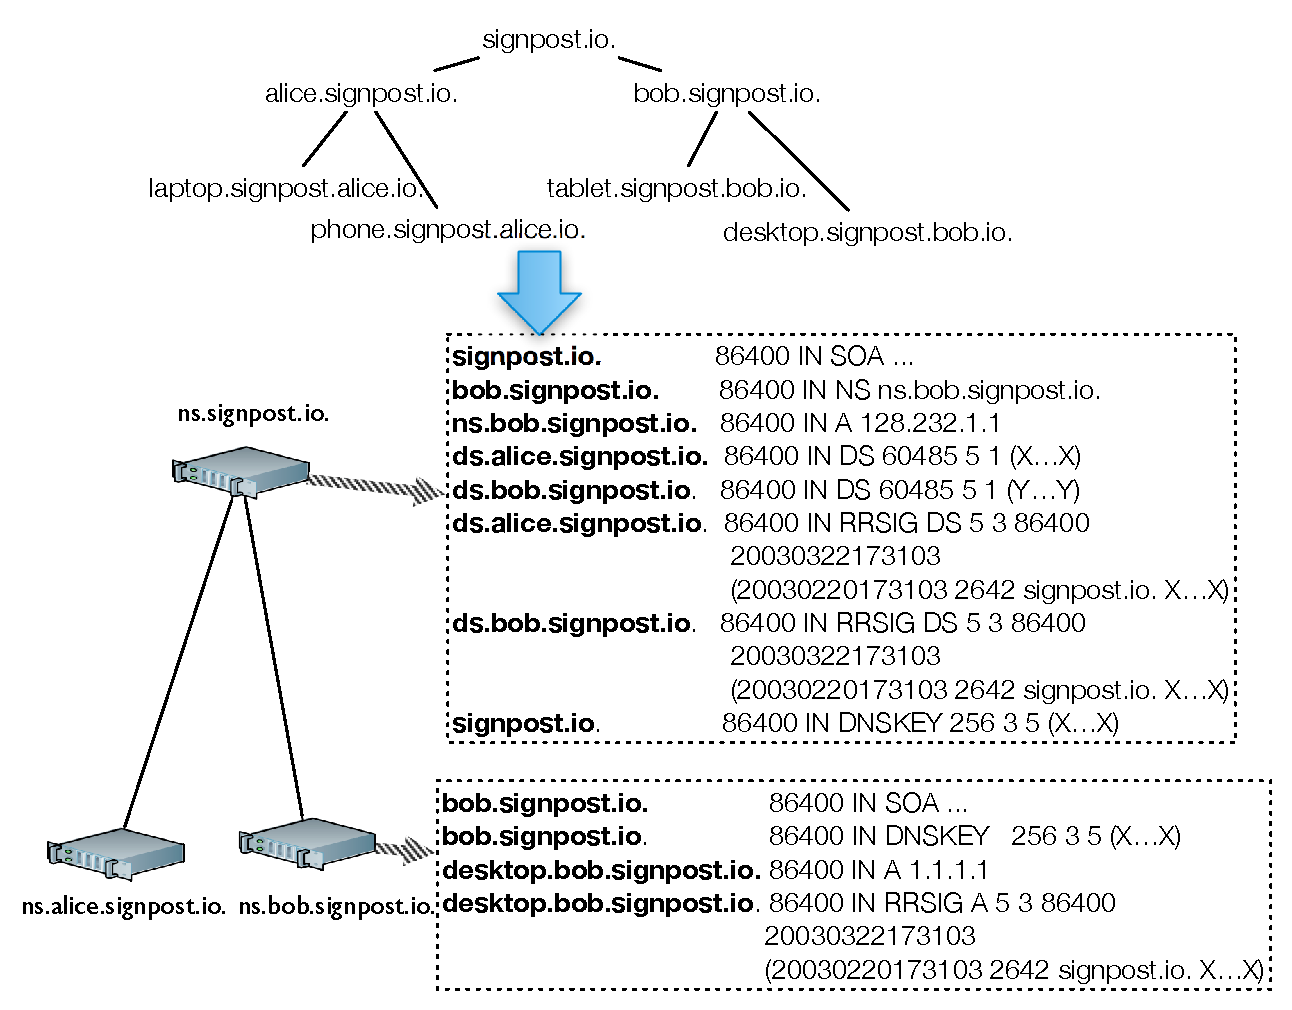
\includegraphics[width=0.8\textwidth]{DNSSEC_hierarchy}
    \caption{DNSSEC key configuration for the io. and bob.io. domains. The io.
      nameserver zone file contains a DS RR with the hash of the bob.io. DNSKEY
      RR and an RRSIG RR signature of the DS RR signed with the DNSKEY of the
      io. domain. bob.io. uses its DNSKEY to sign an A RR for desktop.bob.io.}
  \label{fig:dnssec_hierarchy}
\end{figure}

In the initial definition of the Internet naming service, the protocol provided
very weak security guarantees. In order to enhance the security primitives the
IETF standardised a number of DNS protocol extensions, describe as \dnssec.
\dnssec defines several three RR types~\cite{RFC4034} used to provide a signing
chain that can authenticate DNS records.  We present the authentication
mechanism in Figure~\ref{fig:dnssec_hierarchy}. In essence, a zone signs its
authoritative RRsets using its private key and the RRSIG record type, and then
publishes its public key via a DNSKEY RR to allow resolvers to validate the
RRset signatures.  In addition, the DS RR propagates trust between nameservers.
Following the signing of the root zone, and certain top level domains beneath
it, a chain of trust is formed back to the root, whereby a given resolver can be
certain that the response it has received to a query \emph{is} the correct
response from the authoritative DNS server for the name in question. The
resolver requires, as in the X509 certificate architecture, only a list of
authenticated anchors configured out-of-band of the protocol and injected in the
authentication chain.

In terms of the \signpost system, we have been delegated control of the \fqsn{ }
domain and registered a signing key with the \spsn{.io} domain.  For each user
of the \signpost system, we delegate and authenticate control to a subdomain and
redirect DNS queries to the \signpost Controller of the user personal cloud,
where the user can register its devices. As an example with reference to
Figure~\ref{fig:signpost-arch}, user Alice is granted control of the domain
\fqsn{alice} where she can register her laptop under the domain name
\fqsn{laptop.alice}.  By running a Signpost server, an individual has a globally
accessible authenticated public identity on the Internet via their
public-private key-pair. Using this key-pair, a user can sign and authenticate
messages, bootstrap public key cryptography mechanisms and run key-exchange
mechanisms such as Diffie-Merkle-Hellman~\cite{RFC2631} and derive new
shared private keys between any two devices over unsecure channels.

The base \dnssec RR types, defined in~\cite{RFC4034}, provide a mechanism to
authenticate responses from a nameserver to a DNS resolvers. In terms of
\signpost, we are also interested enabling an authentication mechanism the
requests of a resolver. This enables the server to present a different view
over the resource mappings, depending on the querying entity.  \footnote{{\em
    ``DNS servers can play games. As long as they appear to deliver a
    syntactically correct response to every query, they can fiddle the
    semantics.''---\,RFC3234~\cite{RFC3234}}} \signpost uses the SIG(0) RR type,
defined in~\cite{RFC2931}, which functions as a signature on a request. The
record was introduced in order to allow authorized clients to update RR records
on an authoritative server, while it permits a client also to point to the
signing entity, in order to fit the authentication within the \dnssec key structure. 

% Using DNSSEC here instead of SSL has several important advantages. Firstly,
% DNSSEC has maintained the integrity of its trust chain better than SSL (which
% has a large set of root certificate providers), and has explicit support for
% incomplete trust chains via look aside validation~\cite{RFC5074}.  Secondly,
% DNSSEC has few network dependencies and exploits all of the distributed benefits
% of DNS, such as caching, proxy lookups, and a low-latency protocol.  Lastly, a
% domain also has a single, well-defined owner if registered under a top-level
% domain, whereas URL-based identity schemes such as
% OpenID~\cite{Recordon:2006:OPU:1179529.1179532} depend on trusting the
% underlying owner of the domain for that URL.\todo{will we discuss icann
%   implications of so many new internet names later on?}

%% \subsection{Centralised Named Routing}
%% \label{s:topo1}

\paragraph{Fitting \dnssec in \signpost} In terms of \signpost architecture, we modify DNS
functionality both on the client and the controller of the architecture. On the
controller we develop a programmable DNS server that functions as
an authoritative server for the user domain. The server provides 
\dnssec access to any host in the Internet for the SOA, DNSKEY and NS records of the
domain, signed with RRSIG records on the fly. Additionally, the server
can verify SIG(0) records from queries and translate signed requests from
\signpost clients in Connection Manager requests. A request for an A RR
for domain name \fqsn{laptop.alice}, signed with a SIG(0) record with a
key from host \fqsn{desktop.alice}, will be translated in a connection request
between Alice's laptop and desktop device to the Connection Manager.
In order to enforce liveness of \signpost RR records in the Internet, we set a zero TTL 
value on all RR records, thus disabling any DNS caching.

In the client side of the \signpost architecture, we have developed a local
\signpost-aware DNS resolver. The resolver enhances the typical resolver
functionality by signing \signpost connectivity request. For normal DNS queries,
the resolver will fetch recursively requested records. For RR requests
under the \signpost domain, the resolver augments the query with a SIG(0) record
signed with the private key of the device. 

Using the DNS protocol we are also able to ensure the functionality of the
system when devices are disconnected from the \signpost Controller, while
connected in the same network. \signpost uses DNS-based service
discovery~(DNS-SD)~\cite{RFC6763} in order to enable secure local device
connectivity.  DNS-SD is a specification of DNS RR organisation which enables
efficient service advertisement and browsing and along with
Multicast-DNS~\cite{RFC6762} they establish an efficient local service discovery
mechanism. The combination of DNS-SD and multicast-DNS is currently a widely
used mechanism for service discovery in local networks and supported by most
available operating systems.  The \signpost system registers and advertises on
the host a service record for the \signpost service with name \_sp.\_tcp.local
in the local network with a target of the domain name of the device, along with
an RRSIG RR and the DNSKEY RR of the device, signed with the private key of the
user. Using these records a \signpost client is able to verify a destination
\signpost service and establish a control channel. 
% This way each device in the local network can listen for the service service
% name and once a new node appears, it can verify the validity of the service.
The device will use the service advertisement information when a name lookup is
performed. During a name lookup,  the destination device will function as a
\signpost Controller responsible for the specific device only and employ all the
logic described previously.

% \paragraph{Putting It Into Practice} Having established a secure identity, we
% require the means to signal a communication channel between any pair of a user's
% devices, no matter the middleboxes and other impediments between them. 
% %In this section we discuss how we adopt the increasingly widely deployed
% %DNSSEC~\cite{Friedlander:2007:DPT:1247001.1247004} for device naming, via a
% %Signpost DNS server ``in the cloud'', and a guaranteed route-of-last-resort
% %tunnel from every device to this server.
% 
% %along with a guaranteed \emph{route-of-last-resort} available through Signposts
% %that provides the latter. Where there are many possible such routes, the
% %``best'' should be chosen, ``best'' being, as ever, application dependent. We
% %discuss construction of higher bandwidth, lower latency routess that make
% %better use of localised resources later~(\S\ref{s:topo2}).
% 
% To make this concrete, consider a simple scenario. Alice has a \signpost server
% running in a globally visible location in the public cloud. This serves her
% public key and zone, \fqsn{alice}, with DNSSEC providing a chain of signed
% attestations back to the DNS root that the record has not been tampered with en
% route. Alice has two network-connected devices, her phone and home desktop.  As
% is typical, her phone's 3G network connection is gatewayed by her mobile
% provider and her home computer is behind a NAT. Thus
% none of her devices are readily reachable directly by each other, or by others
% via the Internet.
% 
% Connecting these two devices currently requires Alice to manually configure a
% tunnel at her NAT box, or to run VPN software on her phone. No automatic
% signalling mechanism exists to setup these connections on demand, nor even to
% address the devices by a global name. With \signpost, Alice binds the concrete
% names \spsn{phone} and \spsn{home} to her devices, and runs a publicly visible
% server hosted in a cloud to coordinate their name resolution.
% 
% Establishing a connection between \spsn{phone} and \spsn{home} via the \signpost
% is then relatively straightforward. One client, say \spsn{home}, initiates the
% process by attempting a DNS resolution of \fqsn{phone.alice}. Normal DNS
% mechanisms cause this query to reach Alice's \signpost, which has been delegated
% the zone \fqsn{alice}. It resolves the name \spsn{phone}, causing various
% \emph{tactics} (\S\ref{s:topo2}) to be executed, the result of which is that a
% VPN is established between Alice's phone and computer, and a valid IP address
% endpoint returned in the DNS query.
% 
% \todo{Somewhere in this section we need to mention Signpost Clients and Signpost
%   Servers -- and the difference between `client' devices. Otherwise the
%   distinction gets confusing later in the report.}



\subsection{Security and Key Management} \label{signpost-security}

In order to bootstrap device authentication, \signpost uses a public key
cryptography mechanism integrated with the \dnssec protocol.  \signpost employs
a key hierarchy, which enables the system to control and revoke trust on device
keys in real time. Our key hierarchy relies and extends the key hierarchy
defined by the \dnssec protocol. For a \signpost cloud the user should construct
at least two keys, A {\it Zone Signing Key (ZSK)} and a {\it Device Signing
  Key(DSK)}. ZSK signs the DSK and a signed hash of the ZSK is stored as a
DS RR in the signpost.io name servers, in order to add the key in the global \dnssec
keychain. DSK is used by the controller to sign Device Keys. This differentiation 
of user keys permits a Personal cloud to
have a persistent anchor in the \dnssec key chain. The DSK can be updated
in fixed weekly basis or when a key
compromise is detected, without having to rely in the \dnssec infrastructure to
propagate the updates to other servers. Each device registered with the cloud
must construct a private Device Key when it first joins the system and add the
public key to the Controler device key cache over a trusted channel. The public
key will be signed by the DSK of the Cloud and shared as a DNSKEY RR by the
controller. A device of a \signpost cloud requires only an anchor in the global
\dnssec key infrastructure and it can easily verify the validate of any
\signpost key.  


\section{Evaluation}\label{sec:signpost-evaluation}

In this section we analyse the performance of the \signpost system and its
impact in the functionality of traditional Personal Cloud applications. We,
 present the implementation details of the system
(Section~\ref{sec:sp-implementation}), measure the performance of the
\signpost tactics over the Internet~(Section~\ref{sec:sp-tactic-eval}) and
present a small scale study of the functionality of current application over the
\signpost system. 

\subsection{\signpost implementation} \label{sec:sp-implementation}

\signpost is implemented predominantly in Ocaml and reuses a number of available
protocol libraries. \signpost uses ocaml-dns for DNS server and
client implementations, cyptokit library for cryptographic key manipulation and
ocaml-openflow library for \of controller functionality. \signpost also uses a
portion of C code to implement binding with the OS routing stack. \signpost
provides support for a wide range of platform. We have managed to run \signpost
successfully under Linux and Android,
using the \ovs switch implementation, and under MacOSX, using the userspace
switch implementation provided by the ocaml-openflow library.


\signpost provides support for the following tactics: 
\begin{itemize}
  \item \emph{Direct}: The tactic enables communication path between devices
        over the network without any tunneling mechanism. The functionality of
        the tactic  provides a mechanism to test direct connectivity between the
        two devices over a number of well-known ports and if successful it will
        insert a single \of rule to translate \signpost IP addresses to the
        respective network addresses. 
  \item \emph{\openvpn}: The tactic enables communication paths using the
    \openvpn tunnelling mechanism. During connection, \signpost devices  use
    the \signpost key infrastructure to generate public keys and bootstrap
    the \openvpn authentication mechanism.  Because of some limitation on
    the certificate chain evaluation of OpenSSL, during a connection the
    Tactic generates transient private keys, signed by the user private key,
    while the tactic will inject in the trusted certificate keychain a key
    certificate of the destination device signed by the private key of the
    device. The tactic configure the \openvpn software to expose
    connectivity over an Ethernet TUN/TAP device~\cite{tuntap}, which is
    added under the control of the \of switch where \of packet forwarding
    rules establish full bi-directional connectivity.  
    \todo{Mention OpenVPN ARP cache}
  \item \emph{SSH}:  The tactic enables connectivity of the system using the SSH
    protocol. For this tactic we configure and run a separate ssh daemon on
    every \signpost device. The daemon runs on port 10000 and permits
    key-based authenticated connectivity for tunneling.
    User authentication is ensured by proper manipulation of authorized keys
    on the server configuration. 
    \signpost clients append device public keys
    in the authorized\_key file in an ad-hoc manner, while clients are
    instructed to use the private key of the device upon connection. The SSH
    program is configured to expose TUN/TAP Ethernet interfaces between
    devices, which are added under the control of the \of switch.
  \item \emph{Privoxy}: This tactic enables HTTP request anonymization using 
    the Privoxy~\cite{privoxy} HTTP proxy. In order to achieve this, we have predefined a
    strict configuration of the privoxy software which strips all HTTP headers
    that may leak personal information of the user. In order to establish
    connectivity, the tactic handles TCP flows in a proactive manner. For each
    SYN packet, the tactic install bi-directional  flows, forwarding data from the
    application to the loopback device and the listening port of the Privoxy.

  \item \emph{Tor}: The tactic enables connectivity between devices over the
    Anonymized network of Tor~\cite{dingledine2006}. Tor client software exposes
    a SOCKS proxy on the local machine which can provide TCP connectivity to
    flows over the Tor overlay network. In order to enable bidirectional
    connectivity over the Tor network, the tactic uses the hidden service
    functionality of the system. A node in Tor is able to expose listening
    ports. In order to achieve this, the system uses random domain names under
    the .onion domain to address nodes and it takes advantage of the socks
    protocol capability to embed name lookups in SOCK connection requests.  Upon
    the request for connection over the Tor network, the \signpost client will
    negotiate with the remote device its domain name under the Tor abstraction.
    Upon a SYN packet transmission of the application to the remote device, the
    tactic will initiate a TCP connection with the local SOCKS proxy with a
    request to establish a path between the two devices. In parallel, once the
    TCP connection is established with the local SOCKS proxy, the tactic will
    respond to the initial SYN request with a SYNACK and advertise a zero window
    in order to suppress any further data transmission from the application.
    Once a SOCKS response is returned by the SOCKS proxy, the tactic will either
    respond to the initial TCP flow with an ACK with a non-zero window and
    insert appropriate \of rules to permit connectivity between the two device
    over the SOCKS tunnel, or the client will inject a TCP RST if the SOCKS
    response was unsuccessful. 
  \item \emph{DNS-SD}: This tactic is used to advertise services provided by the
    \signpost devices. DNS-SD~\cite{RFC6763} is a popular mechanism, provided by
    the OS, to advertise available host services in the local network.  The
    tactic doesn't provide any path establishing functionality to applications,
    but it aid the advertisement of host functionality. The Tactic
    implementation intercepts DNS-SD service advertisement and propagate them
    over the control channel, to the other devices of the Cloud. Each \signpost
    client is responsible then to inject DNS-SD multicast packets over the local
    loopback device of the OS and propagates information in the local ZeroConf
    daemon. 
  \item \emph{NAT-punch}: This tactic uses simple packet injection mechanisms in
    order to allow devices to bypass NAT boxes. The
    functionality of this tactic is limited and covers only the cases of
    Full-cone NAT, Address-restricted NAT and Port-restricted NAT, and
    requires that the NAT functionality doesn't perform any stateful packet
    filtering. Nat punching functionality is achieve by using the Controller as
    an intermediate service that can infer the port mappings configuration of
    the NAT-box. On a TCP connection, the server will intercept the SYN
    request, propagate the important TCP header parameters over the control
    channel to the destination device and in parallel will send a SYN packet
    from the device to the Controller in order to infer the port mapping
    applied by the device. On the destination device the \signpost client
    will generate a SYN packet with similar values to the inital SYN packet
    and send the packet to the local listening service over the loopback
    device as well as the Controller of the Cloud. During this processing,
    both ends of the TCP connection hold the connection idle with a zero
    window. Once the exact port-mapping is inferred on the controller, the
    information is propagate to both devices, which will insert
    appropriate \of commands to manipulate source and destination port
    renumbering and notify the end-points to resume data transmission using
    a ACK with a non-zero window size.
\end{itemize}

\subsection{Tunnel Evaluation} \label{sec:sp-tactic-eval}

\begin{table*}
\centering 
\begin{tabular}{|l|c|c|c|c|c|c| }
  \hline
  \multirow{2}{*}{Tactic name} & \multicolumn{2}{|c|}{Direct connectivity} &
  \multicolumn{2}{|c|}{via-cloud connectivity} \\
\cline{2-5}
& setup~(sec) & throughput~(kbps) & latency~(msec) & setup~(sec) &
throughput~(kbps) & latency~(msec) \\
\hline
Direct       & 10 & 94.1 & 1380 & - & - & - \\
Openvpn       & 21046 & 10 & 10 & 21466 & 18700 & 170\\
SSH       & 10 & 10 & 10 & 10 & 10 & 10 \\
tor       & 10 & 10 & 10 & 10 & 10 & 10\\
NAT-punch & 10 & 10 & 10 & - & - & - \\

% iperf -c quorum101.cl.cam.ac.uk  -i 1 -F /dev/urandom -t 60
% fping 172.31.28.49 -e -b 1400 -c 6000 -p 1 -D -s -e -q
\hline
\end{tabular}
\end{table*}

\subsection{Application compatibility}

\section{Conclusions}\label{sec:signpost-conclusion}

\begin{itemize}
  \item This is an elementary approach for Personal Cloud computing. 
  \item A number of issues remain unandressed but can easily fit in the
        \signpost architecture
  \item extending the policy mechanism, we can integrate in a Personal cloud
        devices from other users. Need though to develop a more refined policy
        that will enable the user to control access from devce outside of its
        personal to a subset of the available services. 
  \item Tighter DNS integration of the control protocol.
  \item 
\end{itemize}
%\section{Second Section}
%\markboth{\MakeUppercase{\thechapter. My Second Chapter }}
%and here I write more ...
%
%\subsection{first subsection in the Second Section}
%... and some more ...
%
%\subsection{second subsection in the Second Section}
%... and some more ...
%
%\subsection{third subsection in the Second Section}
%... and some more ...

% ------------------------------------------------------------------------

%%% Local Variables: 
%%% mode: latex
%%% TeX-master: "../thesis"
%%% End: 
